\documentclass[a4paper, 12pt]{article} %%%here01

\usepackage[slovene]{babel}
\usepackage[utf8]{inputenc}
\usepackage[T1]{fontenc}
\usepackage{lmodern}
\usepackage{units}
\usepackage{eurosym}
\usepackage{amsmath}
\usepackage{amssymb}
\usepackage{amsthm}
\usepackage{amsfonts}
\usepackage{mathtools}
\usepackage{graphicx}
\usepackage{color}
\usepackage{url}
\usepackage{hyperref}
\usepackage{enumerate}
\usepackage{enumitem}
\usepackage{pifont}

\definecolor{airforceblue}{rgb}{0.36, 0.54, 0.66}
\definecolor{bostonuniversityred}{rgb}{0.8, 0.0, 0.0}

\newcommand{\Zn}{\mathbb{Z}_n}
\renewcommand{\P}{\mathbb{P}}

\newenvironment{matematika}[1]{
{\underline{\textsc{#1:}}}
}{
}

\setlength{\parindent}{12pt}

\begin{document}
%naslov
\begin{titlepage}
\centering
\textbf{\Huge{Presečišča Bezierovih krivulj}}
\vfill
\textbf{\LARGE{Pristop s subdivizijskim algoritmom}}
\vfill\vfill
\textsc{\Large{Benjamin Benčina}}
\vfill\vfill
\textsc{\large{Univerza v Ljubljani}}

\textsc{\large{Fakulteta za matematiko in fiziko}}

\textsc{\large{Oddelek za matematiko}}
\vfill\vfill\vfill
	
{\large\today}

\end{titlepage}

%kazalo
\tableofcontents
\newpage

\section{Uvod}

Denimo, da imamo dva robota, ki se gibljeta vsak po svoji Bezierovi krivulji. Radi bi izračunali, ali se robota kdaj srečata. Da rešimo problem, bomo očitno potrebovali presečišča teh krivulj, saj če se krivulji ne sekata, se tudi robotka gotovo nikoli ne srečata.

V tem delu bomo obravnavali subdivizijski algoritem za izračun presečišč dveh Bezierovih krivulj. Najprej si bomo ogledali ovojnico množice kontrolnih točk Bezierove krivulje. Natančneje, našli bomo pravokotnik, ki vsebuje vse kontrolne točke. V naslednjem koraku bomo implementirali algoritem, ki nam bo vrnil konveksno ovojnico množice kontrolnih točk, torej najmanjši konveksni mnogokotnik, ki vsebuje vse kontrolne točke. Nato se bomo vprašali, kdaj se dva mnogokotnika sekata. To bo naš kriterij sekanja, če se dve ovojnici ne sekata, se tudi krivulji ne bosta. Nato bomo definirila subdivizijo Bezierove krivulje in implementirali rekurzivni algoritem, ki bo poiskal vsa presečišča.

Poleg osnovne ideje v ozadju posameznega koraka bodo podani tudi sklici na kodne datoteke, ki bodo priložene.

\section{Bezierove krivulje}

Najprej ponovimo, kaj natančno je Bezierova krivulja.\\
\begin{matematika}{Definicija 2.1}
Bezierova krivulja $B\colon [0, 1] \to \mathbb{R}^2$ določena z množico kontrolnih točk $B = \lbrace B_i \rbrace_{i = 0}^n$ je definirana z enačbo
\[ B(t) = \sum_{i = 0}^n b_{i,n}(t)B_i, \]
kjer so $b_{i,n}(t) = \binom{n}{i}t^{i}(1-t)^{n-i}$ Bernsteinovi bazni polinomi.
\end{matematika}

Ta definicija je ekvivalentna definiciji z de Casteljaujevim algoritmom, ki je ne bomo posebej navajali, algoritem pa se nahaja v datoteki \emph{deCasteljau.m}.
\section{Ovojnice}

V tem poglavju si bomo natančneje ogledali dva tipa ovojnic končne množice kontrolnih točk. To sta pravokotnik, ki vsebuje vse kontrolne točke, in konveksna ovojnica. Kasneje si bomo s presečišči ovojnic pomagali pri iskanju presečišč krivulj. Potrebujemo naslednji izrek.\\
\begin{matematika}{Izrek 3.1}
Vsaka Bezierova krivulja je v celoti vsebovana v konveksni ovojnici svojih kontrolnih točk.\\
\end{matematika}
\begin{matematika}{Dokaz}
Izrek sledi direktno iz konstrukcije Bezierove krivulje z deCasteljau-ovim algoritmom. Vsaka točka na Bezierovi krivulji je po deCasteljau-ovem algoritmu konveksna kombinacija kontrolnih točk in zato po definiciji vsebovana v konveksni ovojnici. \hspace*{\fill} $\square$\\
\end{matematika}
\begin{matematika}{Posledica 3.2}
Vsaka množica, ki vsebuje vse kontrolne točke Bezierove krivulje, vsebuje tudi celotno krivuljo.
\end{matematika}

Zadnja posledica nam pove, da za ovojnico lahko uporabimo poljuben lik, ki vsebuje vse kontrolne točke, torej lahko vzamemo računsko najlažjega. Osredotočili se bomo na pravokotnik.

\subsection{Pravokotna ovojnica}
Iščemo torej smiselen pravokotnik, ki bo vseboval vse kontrolne točke Bezierove krivulje. Hkrati želimo, da je dovolj majhen, da ga lahko kasneje uporabimo za kriterij sekanja, ko bomo krivuljo smiselno manjšali.

\begin{figure}[!h]
	\centering
	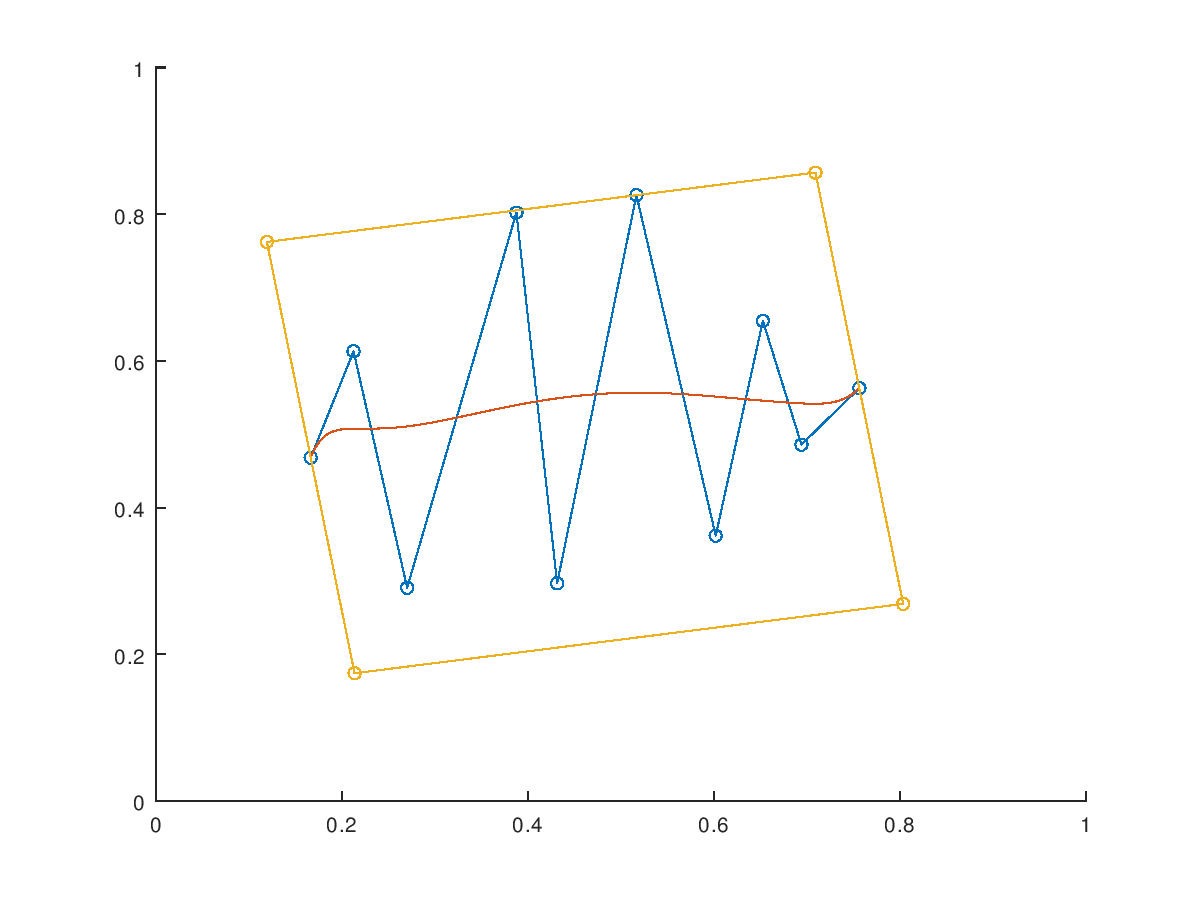
\includegraphics[scale=0.5]{pravokotnik}
	\caption{Pravokotna ovojnica Bezierove krivulje v testnem okolju \emph{testPravokotnik}.}
	\label{fig:pravokotnik}
\end{figure}

Ideja je naslednja:
\begin{itemize}
\item Najdemo dve kontrolni točki $P$ in $Q$, ki imata največjo medsebojno razdaljo.
\item Vektor $s$ od ene do druge točke predstavlja srednjico pravokotnika.
\item Poiščemo tisto izmed preostalih kontrolnih točk, ki ima najdaljšo pravokotno razdaljo do premice, ki jo definirata vektor $s$ in ena izmed točk $P$ in $Q$.
\item Vektor $b$ naj bo vektor te pravokotne razdalje.
\item Oglišča iskanega pravokotnika so potem $P + b$, $P - b$, $Q + b$, $Q - b$.
\end{itemize}


Glavna lastnost tako definiranega pravokotnika je, da je njegova velikost odvisna le od razdalj med kontrolnimi točkami. Če bomo krivuljo torej pravilno manjšali, bomo dobili manjši pravokotnik.

Implementiran algoritem se nahaja v datoteki \emph{pravokotnik.m}. Funkcijo lahko grafično testiramo s pomočjo skripte v datoteki \emph{testPravokotnik.m}.

\subsection{Konveksna ovojnica}
Vseeno pa bi za pravo mero sekanja radi uporabili najmanjšo množico, ki vsebuje vse kontrolne točke, torej njihovo konveksno ovojnico. Za končno množico točk $B$ je to vedno konveksni mnogokotnik, čigar oglišča so urejena podmnožica $K \subseteq B$. Algoritmov za iskanje konveksne ovojnice množice točk je mnogo, vsak s svojimi prednostmi in slabostmi, osredotočili pa se bomo na \emph{Grahamov algoritem} (angl. \emph{Graham Scan}). Razloga za to sta dva. Prvič, ideja algoritma je jedrnata, intuitivna in lahko razumljiva. Drugič, časovna zahtevnost algoritma je med bolj optimalnimi. S preprostim razmislekom lahko utemeljimo, da je hitrost iskanja konveksne ovojnice v optimalnem primeru navzdol omejena s sortiranjem množice točk $B$. Konveksne ovojnice torej ne moremo najti hitreje kot $\mathcal{O}(n\log{}n)$, kjer je $n = |B|$. Časovna zahtevnost Grahamovega algoritma za iskanje konveksne ovojnice pa je približno enaka $\mathcal{O}(n\log{}n)$.



Ideja algoritma je naslednja:
\begin{itemize}
\item Najdemo najbolj levo najnižjo točko $P_0 \in B$.
\item Vse ostale točke razvrstimo po polarnem kotu vektorja $P_i - P_0$, kjer $i = 1, \dots, n$.
\item Deklariramo prazen sklad, na katerega bomo nalagali trenutne kandidate za oglišča konveksne ogrinjače.
\item Sprehodimo se čez urejen seznam točk in preverimo, da se z vsako novo točko premaknemo v nasprotni smeri urinega kazalca. Če to ni res, sklad praznimo dokler ni za trenutno točko to izpolnjeno.
\item Ko pregled končamo, nam na skladu ostane urejen seznam oglišč konveksne ovojnice.
\end{itemize}

\begin{figure}[!h]
	\centering
	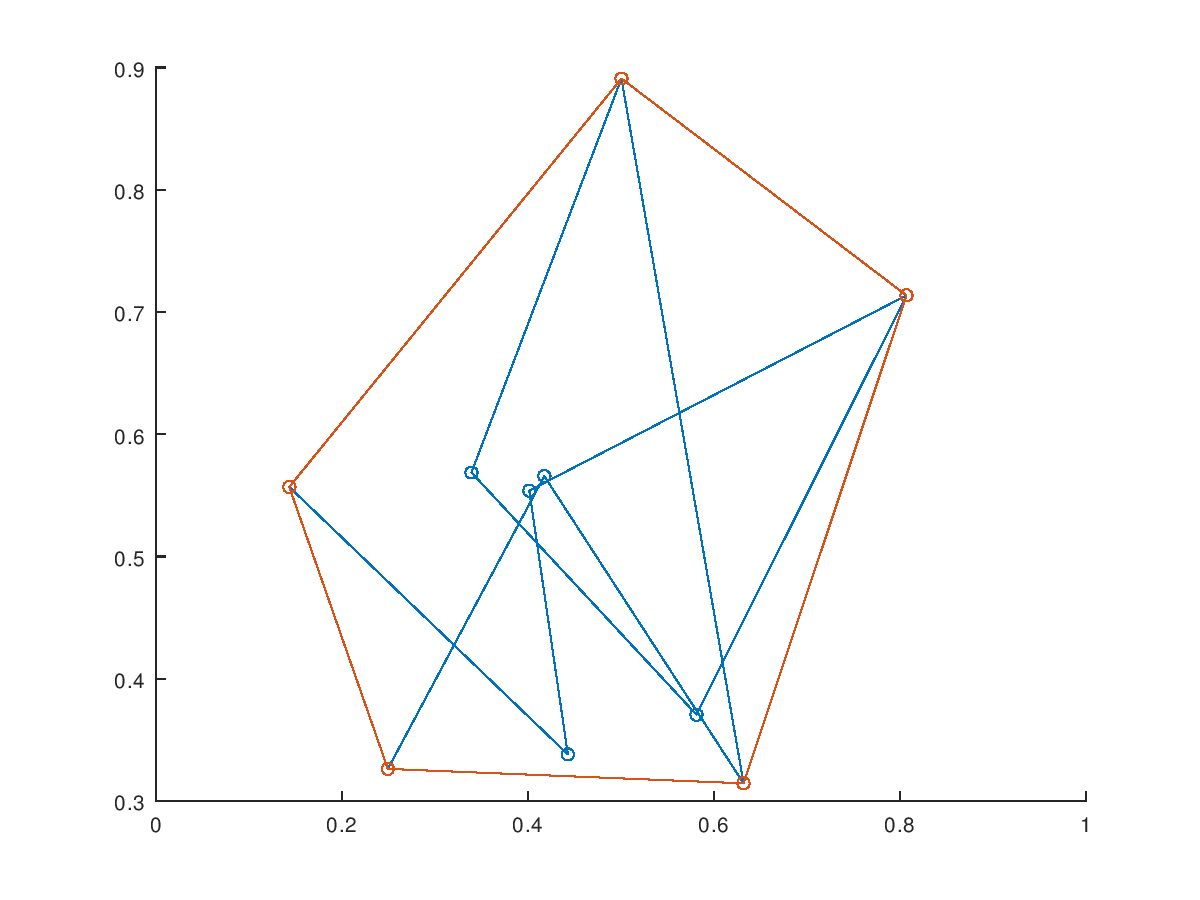
\includegraphics[scale=0.5]{graham}
	\caption{Konveksna ovojnica množice točk v testnem okolju \emph{testGraham}.}
	\label{fig:graham}
\end{figure}

Vredno je omeniti, da je izbira spodnje leve točke popolnoma arbitrarna. Zagotavlja nam le, da bo polarni kot vsakega vektorja $P_i - P_0$, kjer $i = 1, \dots, n$, vedno med $0$ in $\pi$, s čimer se izognemo problemom z negativnimi koti ter poskrbimo, da bo točka $P_0$ vedno oglišče ovojnice. S podobnim argumentom bi lahko izbrali poljubno robno točko in primerno prilagodili sortiranje kotov.


Ideja algoritma je torej, da si izberemo začetno oglišče in nato v nasprotni smeri urinega kazalca tvorimo pozitivno orientiran konveksni mnogokotnik.


Implementiran in dobro komentiran algoritem se nahaja v datoteki \emph{grahamScan.m}, funkcijo pa lahko dalje grafično preizkušate z datoteko \emph{testGraham.m}. Primer je prikazan na sliki \ref{fig:graham}.


Pošteno je še opomniti, da programska jezika MATLAB in Octave že imata implementirano funkcijo \emph{convhull}, ki nam vrne indekse točk konveksne ovojnice množice točk $B$.

\section{Presek mnogokotnikov}

Sedaj, ko smo definirali ovojnice, se lahko vprašamo, kdaj se dve ovojnici sekata. Ker sta oba obravnava tipa ovojnic mnogokotnika, nas bo v tem poglavju zanimalo, natanko kdaj se dva mnogokotnika sekata, torej kdaj imata neprazen presek.\\
\begin{matematika}{Izrek 4.1}
Mnogokotnika $A$ in $B$ imata neprazen presek natanko tedaj, ko se seka najmanj en par njunih stranic ali pa eden vsebuje kakšno oglišče drugega.\\
\end{matematika}
\begin{matematika}{Dokaz}
Če se seka en par stranic mnogokotnikov $A$ in $B$, potem imata očitno neprazen presek.
Zato privzemimo, da se poljubni dve stranici mnogokotnikov $A$ in $B$ ne sekata. Potem je bodisi en vsebovan v drugem bodisi sta si disjunktna. Če je en vsebovan v drugem, je presek kar manjši od obeh pravokotnikov. Če sta si disjunktna, je njun presek po definiciji prazen.

S tem je izrek dokazan.\hspace*{\fill} $\square$
\end{matematika}

To idejo lahko sedaj implementiramo v preprost algoritem, ki vrne $1$, če se podana mnogokotnika sekata, in $0$, če se ne.

Najprej z vgrajeno funkcijo preverimo, če se katero izmed oglišč enega mnogokotnika nahaja v drugem, nato pa v skrajnem primeru preverimo še, če se sekata kateri njuni stranici. Algoritem se nahaja v datoteki \emph{mnogokotnika\_sekata.m}. Uporablja pomožno funkcijo \emph{presek\_daljic}, ki se nahaja v istoimenski datoteki.

\section{Subdivizija Bezierove krivulje}

Recimo, da imamo Bezierovo krivuljo, podano z množico kontrolnih točk $B$, ki je parametrizirana na intervalu $[0, 1]$, radi pa bi dobili kontrolne točke dela krivulje, na katerem parameter teče po intervalu $[0, c]$ za nek $0 < c < 1$. Tej podkrivulji se reče \emph{subdivizija} Bezierove krivulje pri parametru $c$. Naredimo lahko še več, pri parametru $c$ nas zanimajo kontrolne točke dveh podkrivulj: tiste, pri kateri parameter teče po intervalu $[0, c]$, in tiste, pri kateri parameter teče po intervalu $[c, 1]$. Na srečo nam kontrolne točke obeh podkrivulji da de Casteljaujev algoritem pri parametru $c$. Kontrolne točke prvega dela krivulje so prvi elementi vsakega stolpca v algoritemski shemi, kontrolne točke drugega pa zadnji elementi vsakega stolpca, kot ilustrirano na spodnjem diagramu.

\begin{figure}[h]
\centering
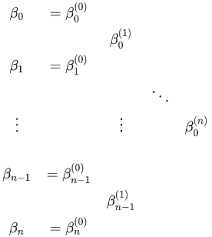
\includegraphics[scale=0.5]{deCasteljau}
\end{figure}

Funkcija, ki sprejme kontrolne točke Bezierove krivulje in parameter $c$ ter vrne kontrolne točke obeh subdivizijskih podkrivulj se nahaja v datoteki \emph{sub\_demo.m}.


\section{Presečišča dveh Bezierovih krivulj}

Zlahka opazimo, da pri subdivizijskem parametru $c = \frac{1}{2}$ krivuljo ravno razpolovimo. Subdivizija nam torej omogoča, da na krivuljo apliciramo bisekcijo, s tem pa si bomo pomagali pri iskanju presečišč. Ideja subdivizijskega algoritma za iskanje presečišč je torej naslednja:
\begin{itemize}
\item Okoli vsake od krivulj naredimo ovojnico.
\item Če se ovojnici ne sekata, opustimo iskanje.
\item Če pa se ovojnici sekata, naredimo bisekcijski korak. Izračunamo subdivizije krivulj pri parametru $c = \frac{1}{2}$ in rekurzivno ponovimo prvi korak na vseh možnih kombinacijah podkrivulj.
\item Če sta obe ovojnici manjši od v naprej določene tolerance, dodamo središče ene od njiju v množico presečišč.
\end{itemize}

\begin{figure}[h!]
	\centering
	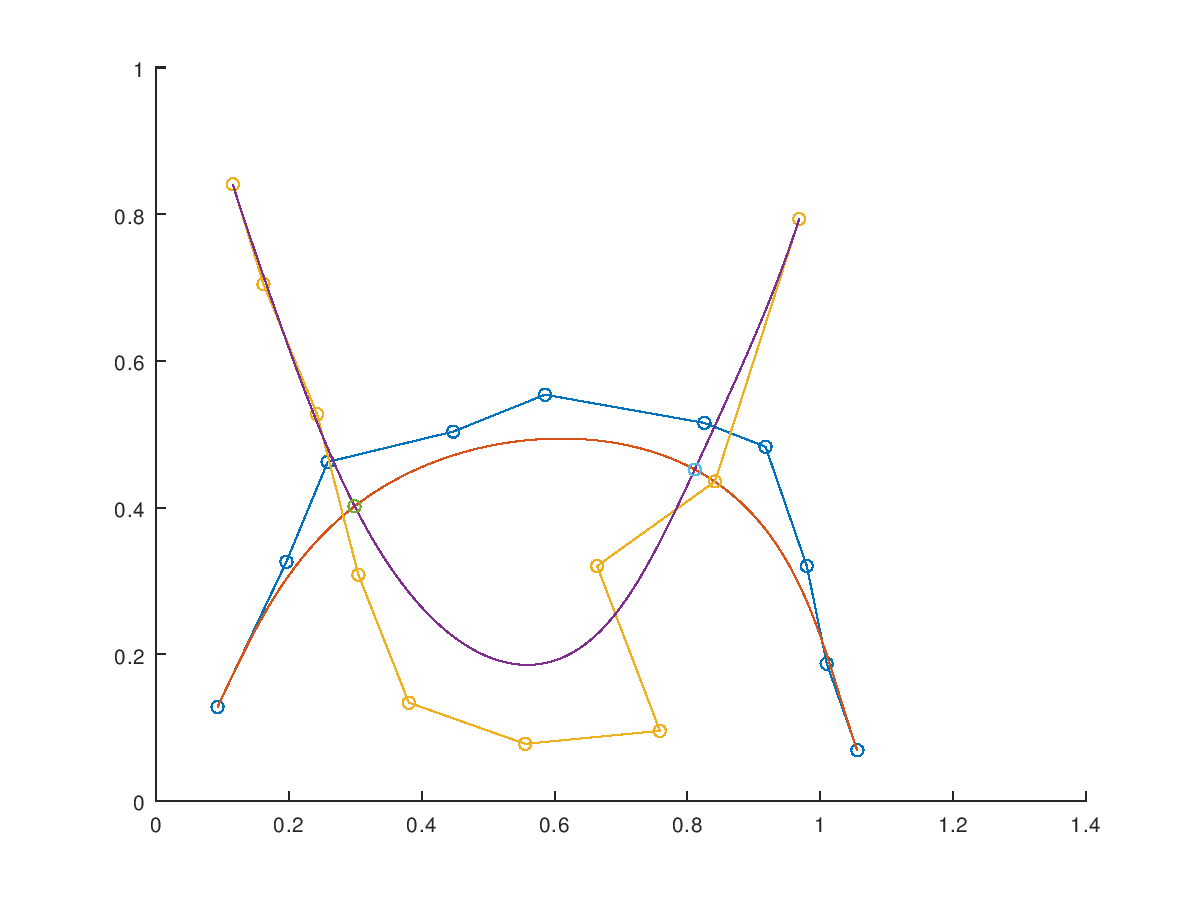
\includegraphics[scale=0.55]{konv}
	\caption{Presečišči Bezierovih krivulj v grafičnem testnem okolju \emph{test\_konv}.}
	\label{fig:konv}
\end{figure}

Rekurzivna algoritma za pravokotno in konveksno ovojnico sta implementirana zaporedoma v datotekah \emph{pravokotni\_bezier.m} in \emph{konveksni\_bezier.m}.
Zraven sta dodani še datoteki \emph{test\_prav.m} in \emph{test\_konv.m}, kjer lahko s pomočjo grafičnega vmesnika testiramo algoritem za pravokotno oziroma konveksno ovojnico.
Slika \ref{fig:konv} tako jasno prikazuje kontrolne točke Bezierovih krivulj, obe krivulji ter označeni obe presečišči. Če bi namest okolja \emph{test\_konv} uporabili okolje \emph{test\_prav}, bi dobili podobno sliko. V konzoli so se izpisale tudi koordinate presečišč.


\section{Zaključek}

Kdaj se torej robota srečata? Z gotovostjo lahko trdimo, da se ne srečata, če se krivulji, po katerih potujeta, ne sekata. V tem primeru bo množica presečišč, ki jo vrne algoritem, prazna. Če pa se Bezierovi krivulji sekata, se robota seveda ne srečata nujno. Primerno moramo prilagoditi njune hitrosti, kar naredimo z reparametrizacijo Bezierove krivulje.

V algoritmu je seveda prostor za izboljšave in pomisleke. Vprašamo se lahko na primer, katero točko nominirati za presečišče, ko sta obe ovojnici po velikosti pod določeno toleranco. Tako pri pravokotni kot pri konveksni ovojnici smo izbrali kar središče ene izmed njiju, zagotovo pa bi bilo bolj korektno izbrati središče preseka ovojnic. Razlog za našo izbiro je, da je središče ena izmed računsko najmanj zahtevnih opcij. Poleg tega je napaka te izbire sprejemljivo majhna, saj se središči obeh ovojnic nahajata znotraj tolerance, ko sta ovojnici dovolj majhni.

Pojavi se tudi vprašanje, ali smo res izbrali računsko najmanj zahtevno ovojnico. Če bi si za ovojnico na primer izbrali krog s središčem v težišču kontrolnih točk in radijem enakim razdalji do od težišča najbolj oddaljene točke, bi bilo preverjanje preseka ovojnic gotovo lažje. Le pogledali bi razdaljo med središčema krožnih ovojnic in jo primerjali z vsoto radijev.
Vsekakor pa je res, da je natančnost algoritma večja, če pri istih kontrolnih točkah izberemo tesnejšo ovojnico, nobena ovojnica pa v primeru Bezierovih krivulj ni za to bolj primerna kot konveksna.

\begin{thebibliography}{9}
\bibitem{bib:lol} kk
\end{thebibliography}

\end{document}